\chapter{Methodology}

\section{Data}
\subsection{Processing}
\subsubsection{Stock Returns}
To obtain stock market returns for Lloyd's, Tesco, Rolls Royce and Vodafone, I used Python 3.9 \cite{Python3} and the Pandas \cite{pandas} library to interact with the Yahoo Finance API. I was specifically working with the closing price (price at the end of the trading day) and the data span from the first trading day in 2017 to the last in 2020. To calculate continuous daily returns I used the formula:
$$
r_t = ln({close}_t) - ln({close}_{t-1})
$$
I chose the continuous daily returns instead of the discrete returns because of the mathematical ease of temporal aggregations for multi-period continuous returns are simply the sum of the logarithmic returns. Take for example k-periods: $r_t(k) = ln(P_t) - ln(P_{t-k})$. I chose to use a simple tool like the Yahoo Finance API over a real time data feed such as Refinitiv because I used simple closing prices of years prior historical stock market data. If I was planning analysis of high frequency time periods, I surely would have used it, but this was easier to implement to the models and has greater opportunity for repeatability by others as Yahoo Finance is free. 

\subsubsection{Irithmics Data}
Unlike simple closing prices of a stock, the data provided by Irithmics arrived in a much more complex way. These data were delivered in comma separated value (.csv) format, that for each company in the FTSE 100, and each trading day in 2020, included a derived discrete probability density, indexed with between 75 and 80 days, describing the probability the deep learning algorithm assigned of a short/sell by the group of funds. $\mathbf{Figure 4.1}$ contains a visual example of what the files for date index January, 26th look like. As this is akin to a probability density, the values on each day will sum to one. 

\begin{figure}[H]
\centering
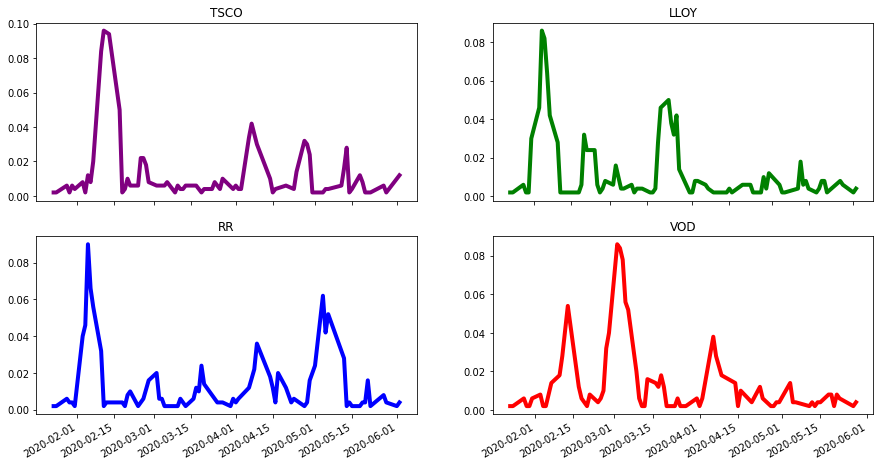
\includegraphics[scale = 0.45]{images/irithmicsprobs.png}
\caption{January 26th Irithmics Probabilities Example}
\label{fig: Irithmics Plot}
\end{figure}

\subsection{Exploratory Data Analysis}
\subsubsection{Stock Returns}


Before building and training any time series models, I first needed to understand and summarise the properties of each of the chosen companies continuous returns. This was guided by the properties of financial asset returns introduced in $\mathbf{Section~1.2.2}$. Because this research is directly focused on volatility, my first step was to obtain the sample standard deviation of each stock's returns, and plot it over the absolute value of those returns $\mathbf{Figure~4.2}$. I assessed the absolute value of the returns rather than the raw value for ease of visualization. The aim of these plots were to evaluate whether or not the returns showed signs of time varying volatility, and volatility clustering. It was immediately apparent that all four stock's returns visually displayed features of both. 

\begin{figure}[hbt!]

\begin{subfigure}{.49\linewidth}
  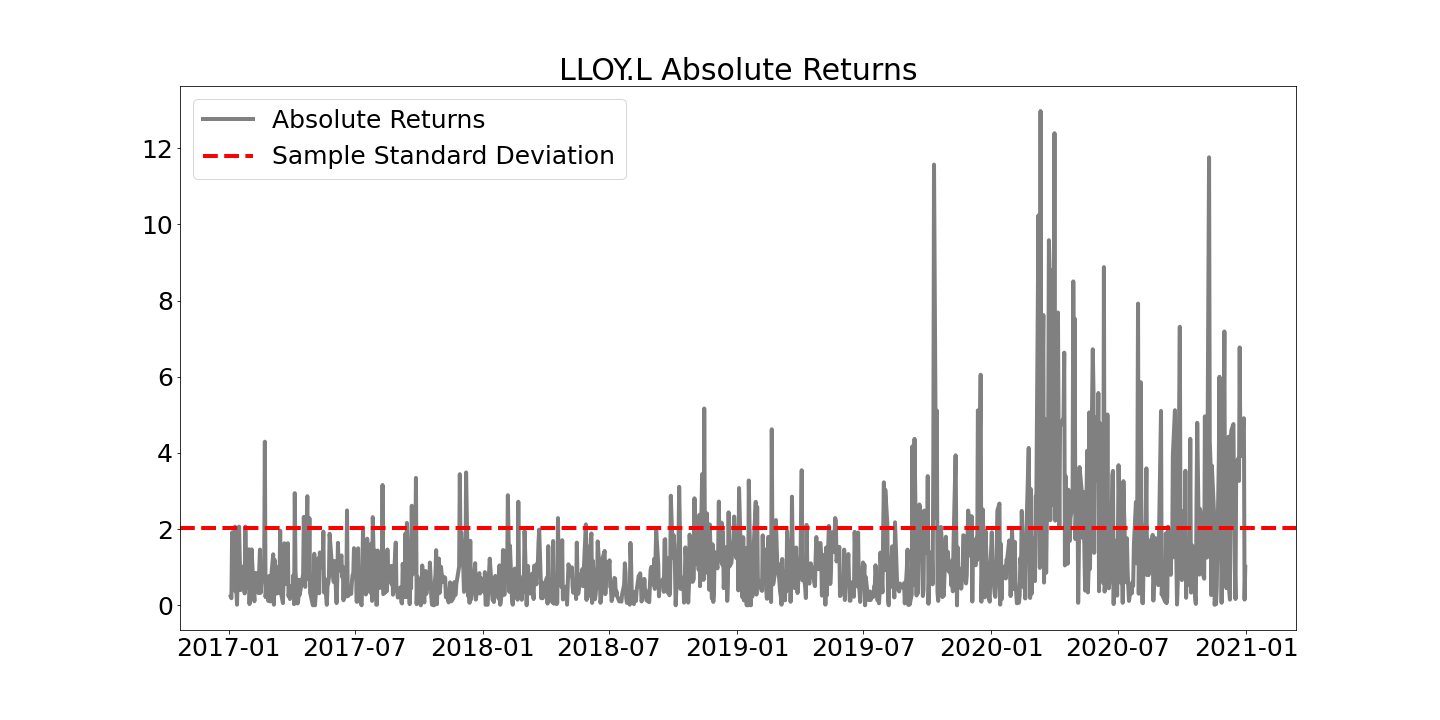
\includegraphics[width=\linewidth]{images/Exploratory/plot 1.png}
  \caption{LLOY}
  \label{A}
\end{subfigure} % <-- "\hfill"
\begin{subfigure}{.49\linewidth}
  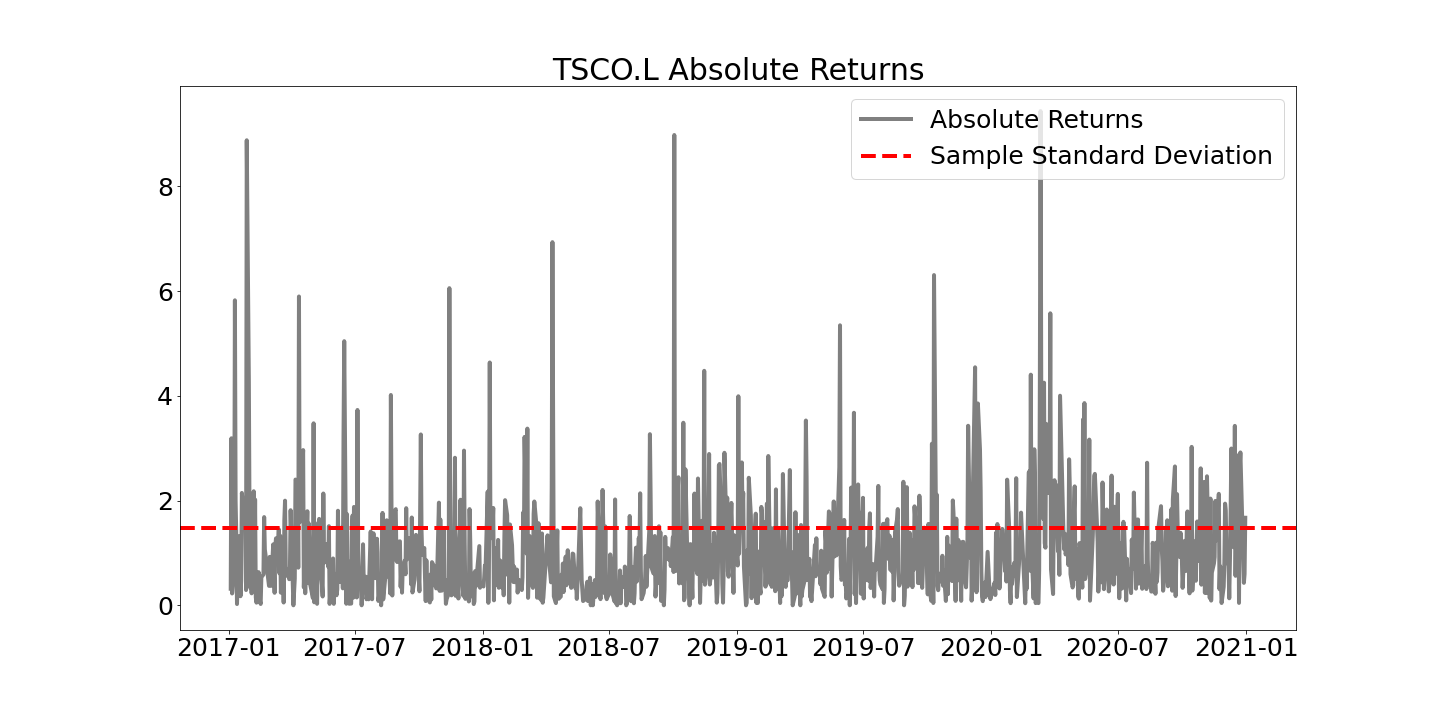
\includegraphics[width=\linewidth]{images/Exploratory/plot 2.png}
  \caption{TSCO}
  \label{B}
\end{subfigure}

\medskip % create some *vertical* separation between the graphs
\begin{subfigure}{.49\linewidth}
  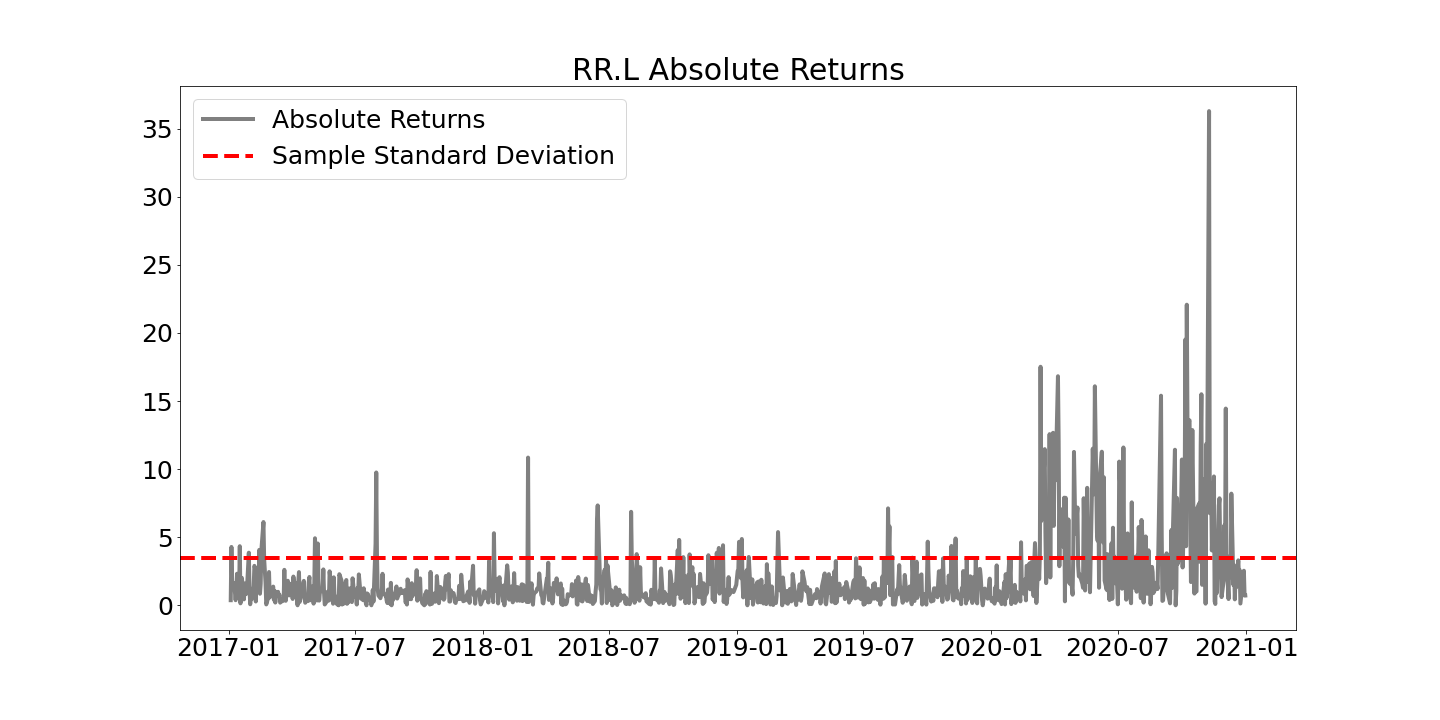
\includegraphics[width=\linewidth]{images/Exploratory/plot 3.png}
  \caption{RR}
  \label{C}
\end{subfigure} % <-- "\hfill"
\begin{subfigure}{.49\linewidth}
  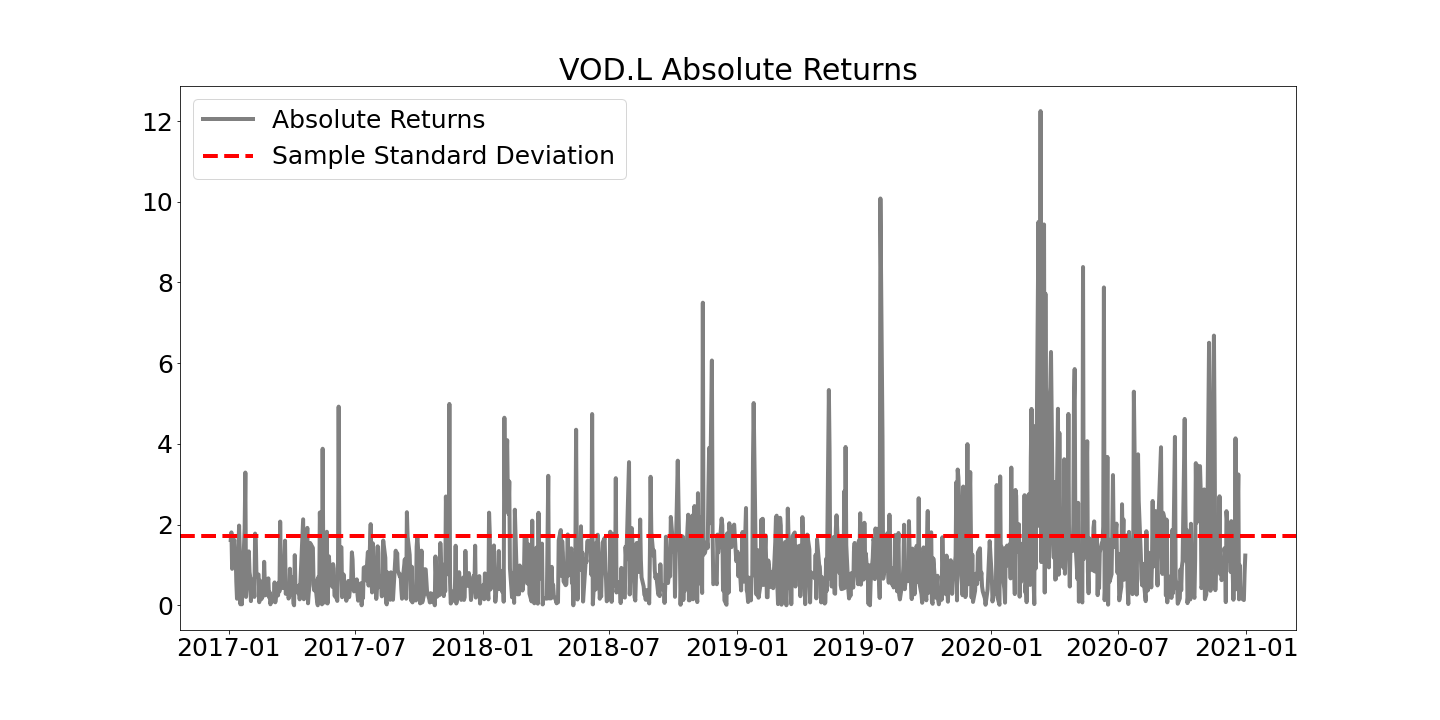
\includegraphics[width=\linewidth]{images/Exploratory/plot 4.png}
  \caption{VOD}
  \label{D}
\end{subfigure}
\caption{Returns v Sample Standard Deviation}
\end{figure}
The next step in exploration was to identify the distribution of the returns. The first and second properties explained that the distribution of the returns should show more probability mass in the tails, as well as having a higher peak than a normal distribution. I implemented $\mathbf{Figure~4.3}$ by using the 'Fitter' Python library. This library implements a kernel density estimation, histogram, as well as overlays other common distributions over the sample data. The distributions are fit using maximum likelihood estimation. Each of the four stocks exhibited the properties of distributions of asset returns differently, following different distributions. Nonetheless, the outcomes were all encouraging and prompted me to continue with the analysis. 

\begin{figure}[hbt!]

\begin{subfigure}{.49\linewidth}
  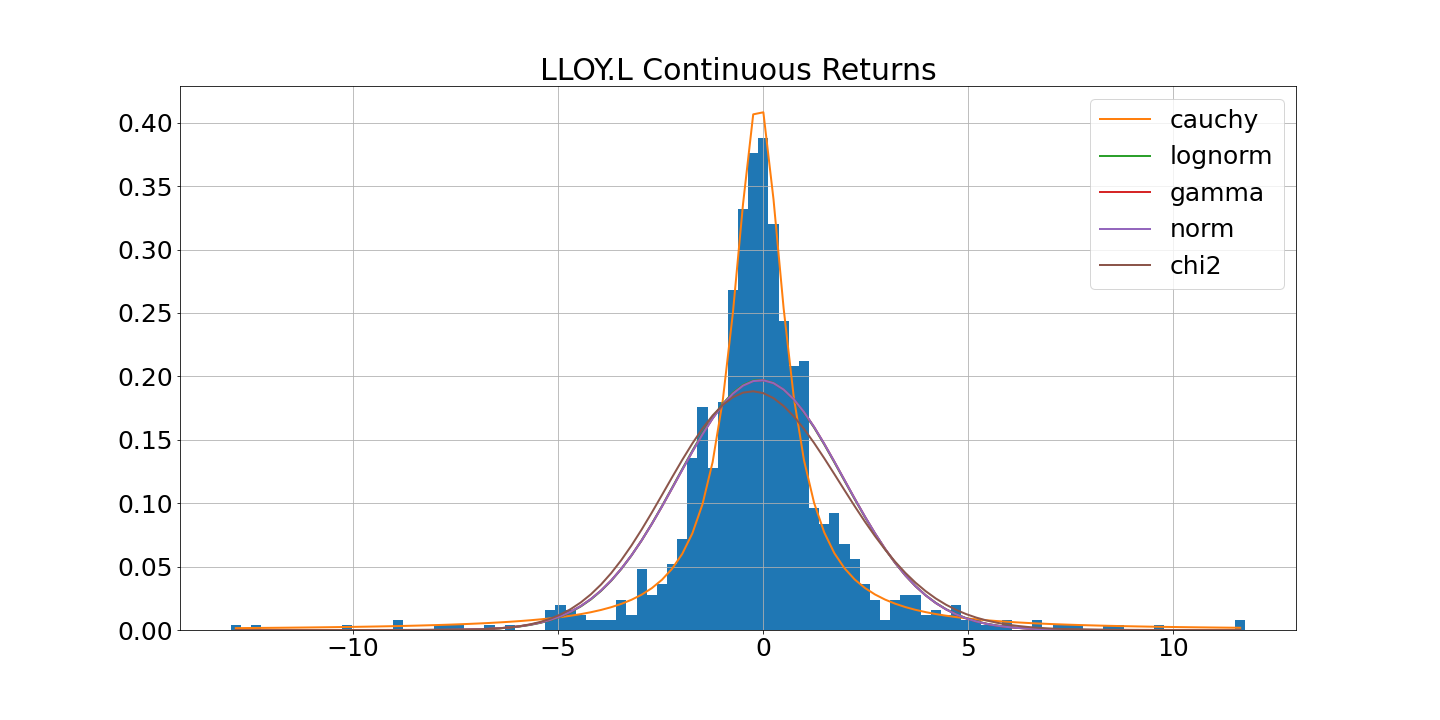
\includegraphics[width=\linewidth]{images/returnDist/plot 1.png}
  \caption{}
  \label{MLEDdet}
\end{subfigure} % <-- "\hfill"
\begin{subfigure}{.49\linewidth}
  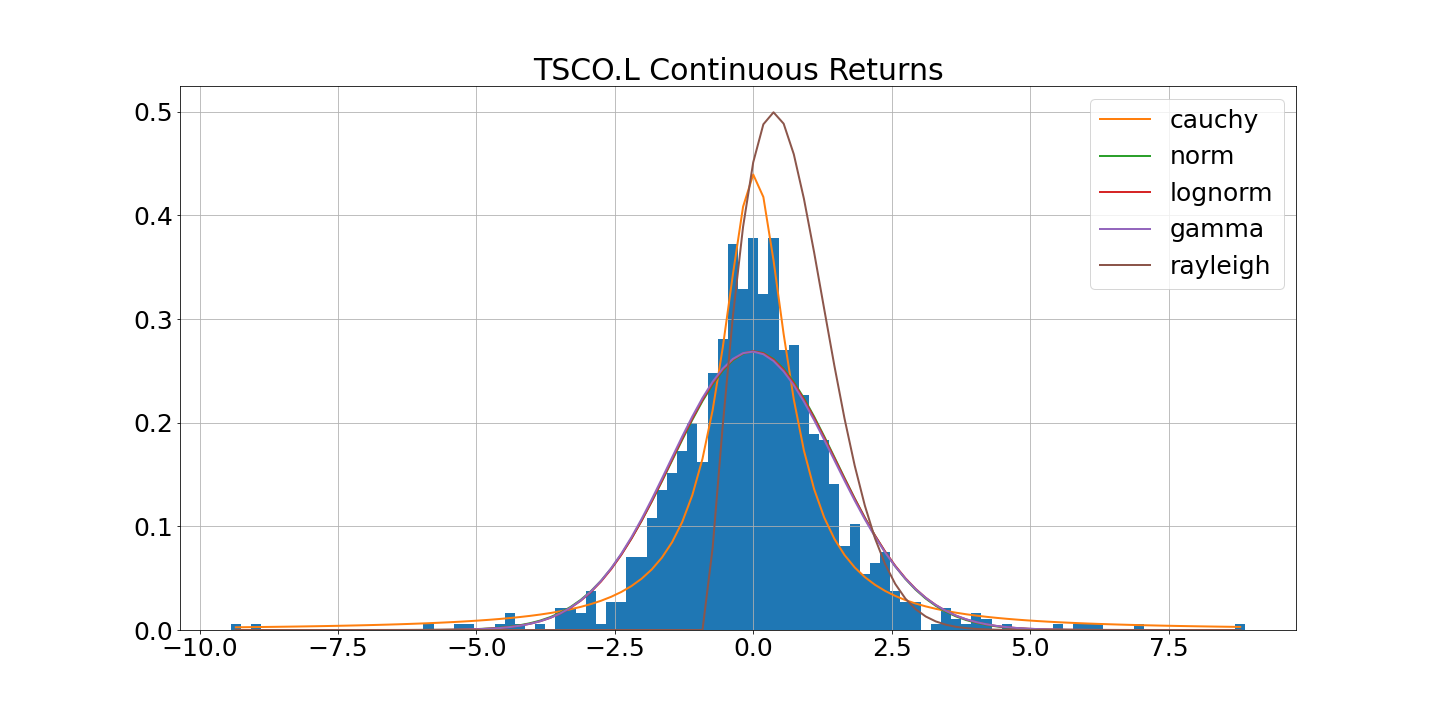
\includegraphics[width=\linewidth]{images/returnDist/plot 2.png}
  \caption{}
  \label{energydetPSK}
\end{subfigure}

\medskip % create some *vertical* separation between the graphs
\begin{subfigure}{.49\linewidth}
  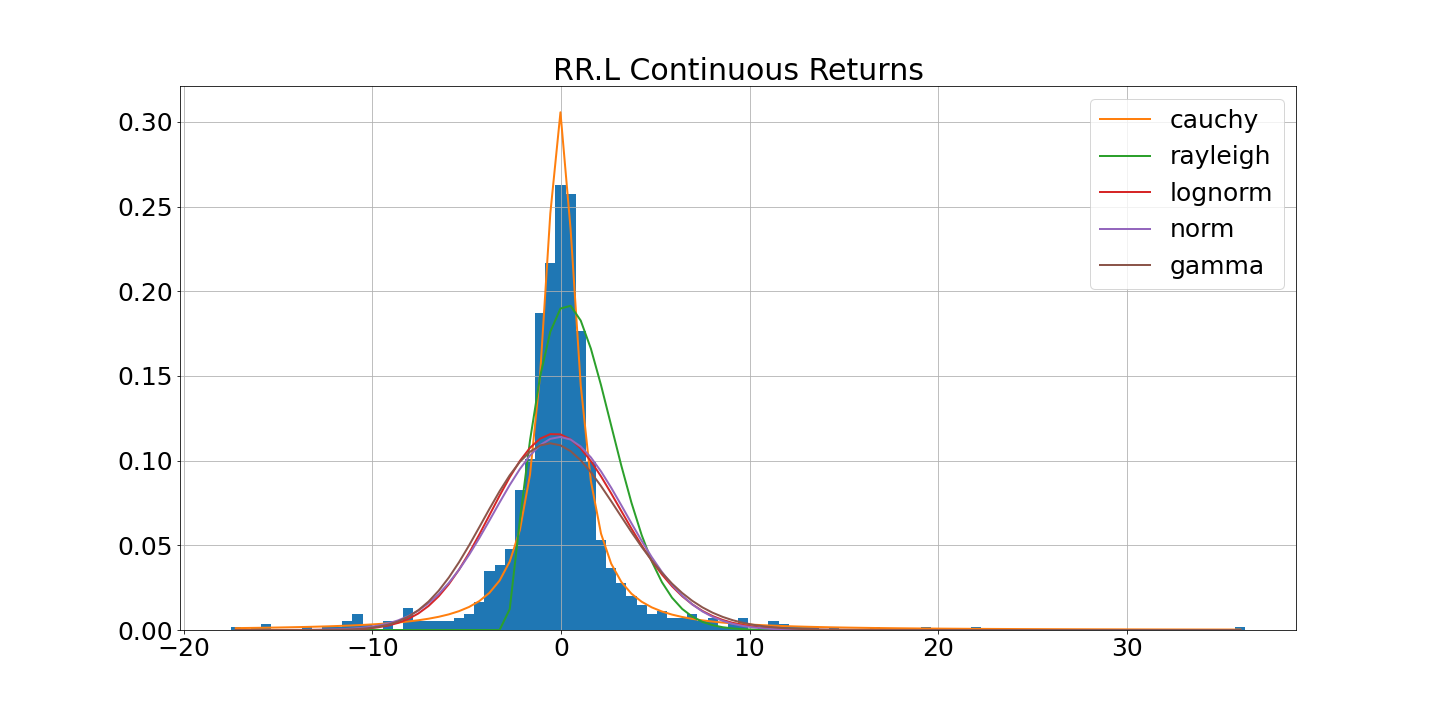
\includegraphics[width=\linewidth]{images/returnDist/plot 3.png}
  \caption{}
  \label{velcomp}
\end{subfigure} % <-- "\hfill"
\begin{subfigure}{.49\linewidth}
  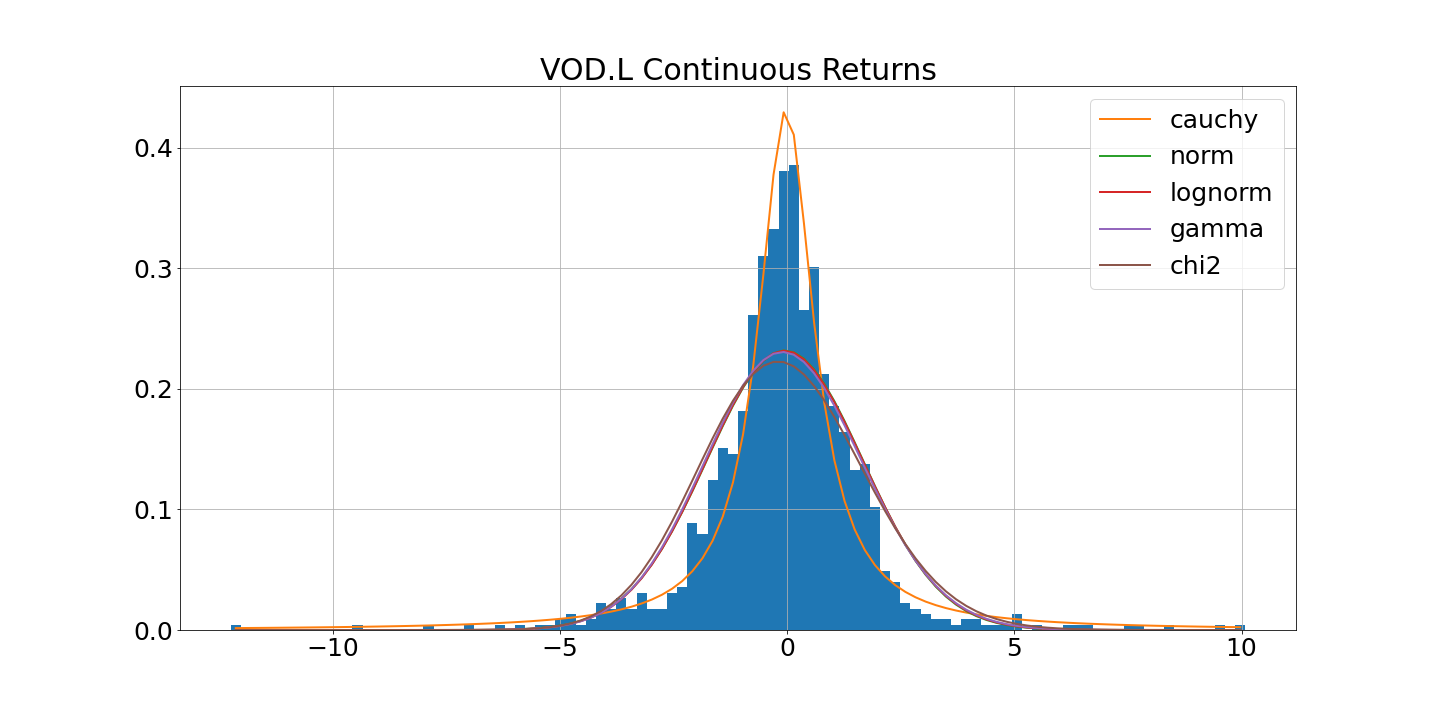
\includegraphics[width=\linewidth]{images/returnDist/plot 4.png}
  \caption{}
  \label{estcomp}
\end{subfigure}
\caption{Returns Distribution}
\end{figure}

The next step was to evaluate the third property of correlation. Since asset returns are said to have minimal to no autocorrelation in continuous returns, but significant autocorrelation in absolute or squared returns \cite{Popov2022}, I transformed the data into squared returns, and plotted the partial autocorrelation function outcome for Lloyd's as an example in $\mathbf{Figure~4.4}$. The plots visually displayed minimal to no autocorrelation between raw returns, but significant partial autocorrelation in squared returns. This is very important to see, as intutively, this is illustrating how, for example, the returns of a stock today, are significantly dependent on the returns of the past 1-3 days. For conditional volatility models such as $\mathbf{GARCH}$, this is of utmost necessity, as explained in $\mathbf{Section~3.2.2}$ the model depends on a specified number of days prior standard deviation and value in the time series. 
  
\begin{figure}[H]
\centering
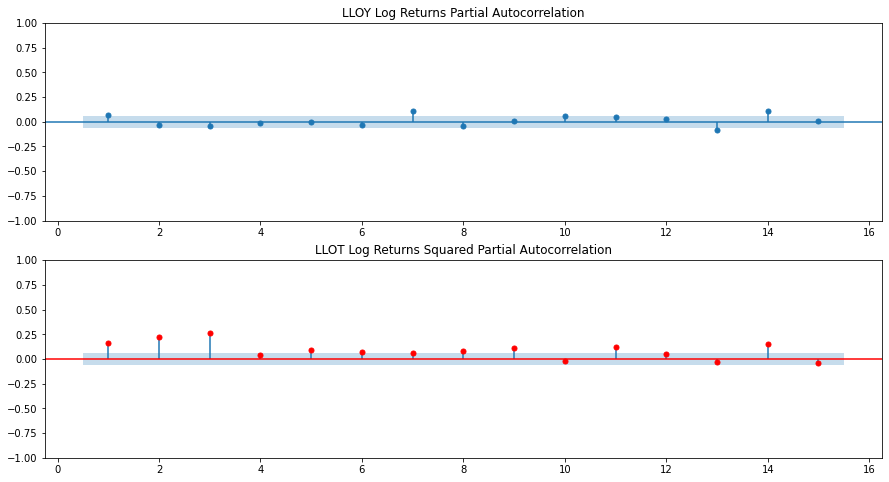
\includegraphics[scale=0.45]{images/PACF.png}
\caption{PACF: Normal v Squared Returns }
\label{fig: Returns v Squared}
\end{figure}

\subsubsection{Irithmics}
The exploration of Irithmics data posed a greater challenge. As these data are non-common and had no prior properties, a more creative approach had to be undertaken. For starters, I returned to $\mathbf{Figure~4.1}$, to get a sample visual representation of the properties of the data. It appeared there were signs of seasonality, or recurring external influences such as economic news or portfolio re-balancing. Something I had to take into great account when evaluating these data was trying not to over-fit models or ideas given the shape of one day's data. Each stock contained between 1-100 predictions for the same trading day, therefore keeping the analysis as generalisable as possible was paramount.    

Preprocessing these data posed two significant challenges: 1) generalisation, 2)formatting. As generalisation has already been discussed, the formatting issue needed to be remedied as fitting a conditional volatility model with an exogenous covariate works similarly to a regression model. The datasets have to be of the same length, and in time series the indices have to match. This meant I had to find a way to aggregate the already aggregated Irithmics probabilities, such that each stock only had one probability of short selling for each trading day. I completed this by implementing a weight decaying algorithm. This algorithm grouped the forecasts for each trading day (between 1-100 observations), and assigned a relative weight based on its temporal location. For example: the short/sell probability for March 25th has a prediction from all days January 1st - March 24th. To aggregate these forecasts, my goal was to mimic the concepts used in $\mathbf{GARCH}$ models, and transform the data into a single, univariate time series: the weight of the probabilities decayed based on its distance from the trading day, i.e. January 10th's prediction carries a lesser weight than March 10th's prediction for March 24th. The outcome of this algorithm is shown in $\mathbf{Figure~4.5}$ and the code can be found in the appendix. 


\begin{figure}[H]
\centering
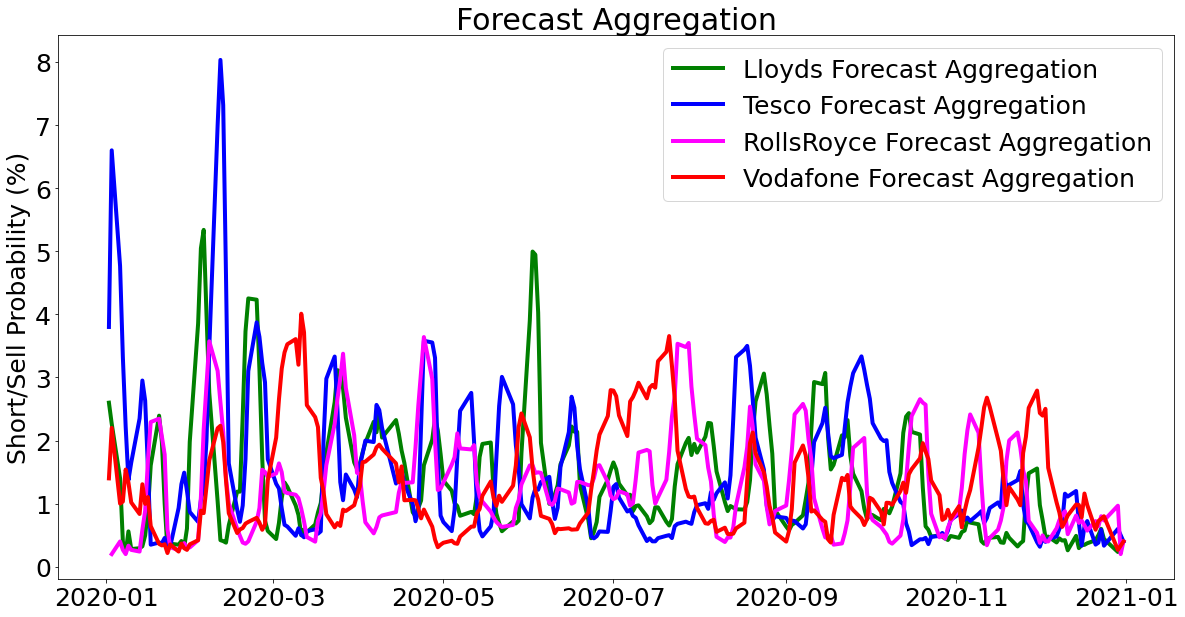
\includegraphics[scale=0.35]{images/Exploratory/forcAgg.png}
\caption{Irithmics Forecast Aggregation}
\label{fig: Irith Forecast Agg}
\end{figure}


\section{Model Fitting}
\subsection{Strategy}

When approaching the fitting and training of models I took a very structured approach. This was because each portion of the project directly built on the outcomes of the prior model. The necessity for consistency across univariate models and models with exogenous covariates cannot be understated as the comparison and impact of the addition of new information had to be the only change, otherwise there would be other factors affecting the forecasted values. The strategy was as follows:

\begin{enumerate}
    \item Implement grid search algorithm to search across combinations of parameters and hyper parameters
    \item Fit many models through algorithm for each stock without the exogenous covariate of Irithmics data
    \item Pick the best model based on Akaike Information Criterion (AIC)
    \item Fit a Dynamic Conditional Correlation (DCC) Model to GARCH Volaility and Irithmics Probabilities
    \item Fit the same model with an exogenous covariate
    \item Forecast last 25 trading days of 2020
    \item Compare generalisation error (MSE MAE)
\end{enumerate}

\subsection{Fitting}
Before I fit any models, I first created a holdout data set in order to retain, albeit small, very important out-of-sample (OOS) data. This data is important because the training and fitting of the models cannot be done with a dataset, and then predict already seen data. These models hopefully can be as generalised as possible, and when fed in new data for future events will have predictive accuracy. Since the sample size was quite small, only one year, the holdout or test data was 25 trading days, about the month of December, 2020. This data is interesting because in the United Kingdom at the time, there was great uncertainty around the next lockdown which inevitably came, and therefore had high potential for greater levels of volatility. 

\subsubsection{Univariate}
To search for the best model, I implemented a grid search algorithm in Python. A grid search's goal is to find optimal hyperparameters in a model, based on a specified loss function. In this case, the available hyperparameters were: Volatility (GARCH/EGARCH), the associated lags (p,q), and the residual distribution (students-t, skewed-t). The chosen loss function is the Akaike Information Criterion (AIC) which is calculated by $$ AIC~=~2(K) - 2ln(L)$$ where $\mathbf{K}$ is the number of parameters and $\mathbf{L}$ is the likelihood. This loss function penalises more complex models as I look to minimise the AIC value. Based on this specification, the algorithm fit 72 different univariate models and returned a list of the top five and bottom five combinations based on this criterion $\mathbf{(Figure~4.6)}$.
\begin{figure}[hbt!]
\begin{subfigure}{.49\linewidth}
  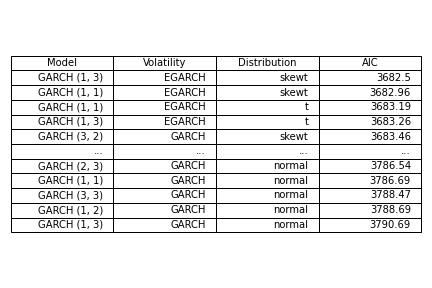
\includegraphics[width=\linewidth]{images/modelFit/stockLLOY.L.png}
  \caption{LLOY}
  \label{fig:A}
\end{subfigure} % <-- "\hfill"
\begin{subfigure}{.49\linewidth}
  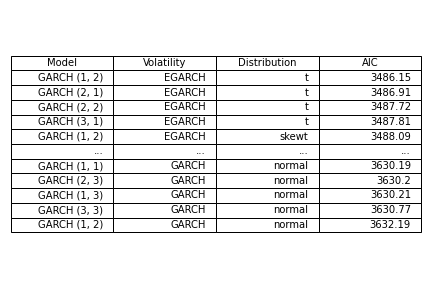
\includegraphics[width=\linewidth]{images/modelFit/stockTSCO.L.png}
  \caption{TSCO}
  \label{fig:B}
\end{subfigure}
\medskip % create some *vertical* separation between the graphs
\begin{subfigure}{.49\linewidth}
  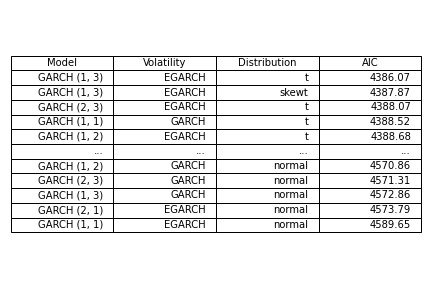
\includegraphics[width=\linewidth]{images/modelFit/stockRR.L.png}
  \caption{RR}
  \label{fig:C}
\end{subfigure} % <-- "\hfill"
\begin{subfigure}{.49\linewidth}
  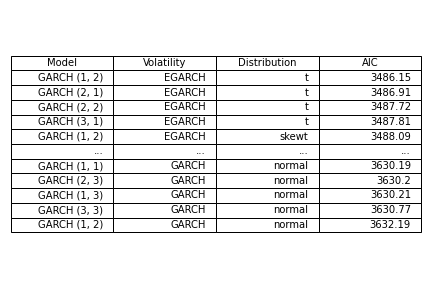
\includegraphics[width=\linewidth]{images/modelFit/stockTSCO.L.png}
  \caption{VOD}
  \label{fig:D}
\end{subfigure}
\caption{Grid Search}
\end{figure}

\subsubsection{Dynamic Conditional Correlation}
While the equations are quite complex, implementing this in Python was rather manageable. Though no available libraries, the researcher by the alias: \cite{DirtyQuant} implemented this in their own project, which I used as a guide. The model took the stock returns and Irithmics probabilities as input, runs a univariate $\mathbf{GARCH}$ model on each series to obtain a conditional volatility estimate, then takes the conditional volatilities as input, into the DCC equation. For each stock and probability pair, the output is a single series containing the Dynamic Conditional Correlation $\mathbf{Figure~4.7}$. The DCC gives information on the dynamic relationship between the two variables, and I hoped to see greater correlation in times of high volatility, which would prompt the model to have an increase in forecast accuracy since I will be fitting the Irithmics data as an exogenous regressor, a linear relationship would show itself here. 

\begin{figure}[H]
\centering
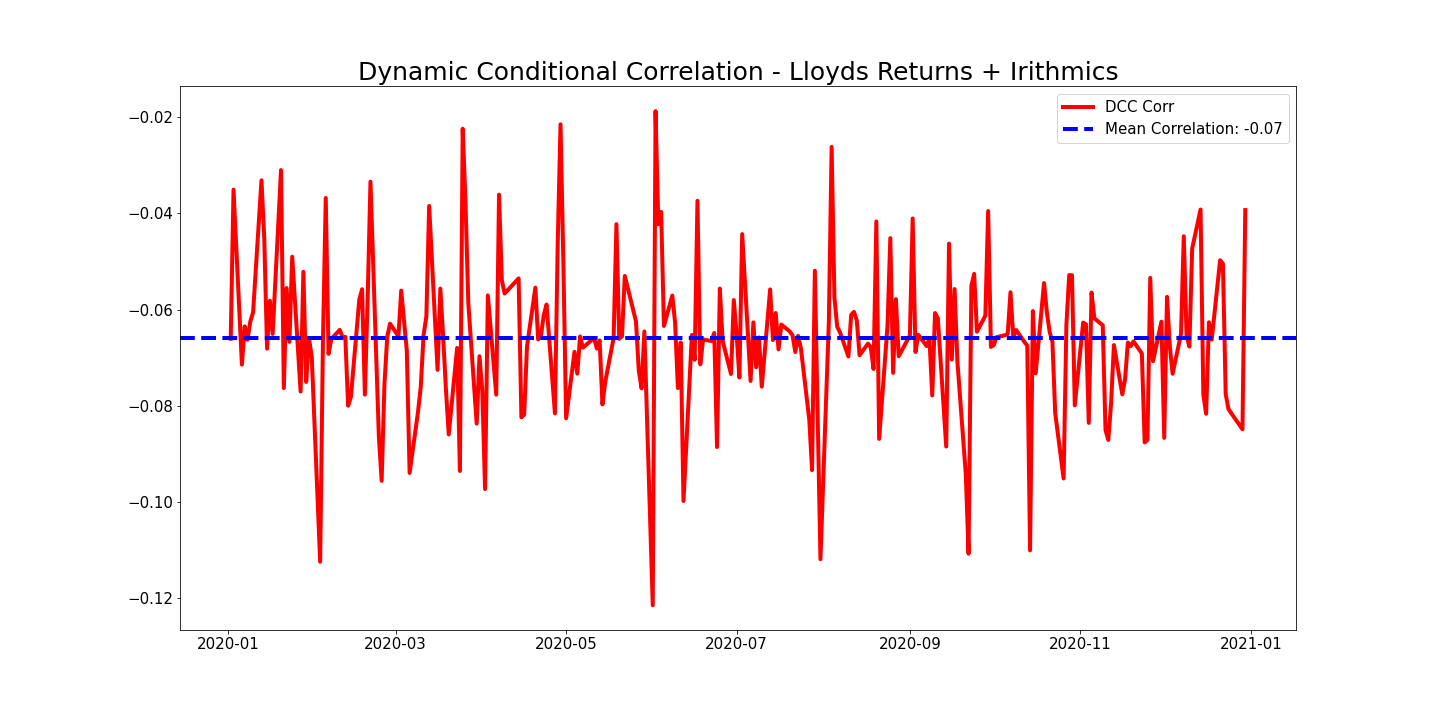
\includegraphics[scale = 0.30]{images/dcc/plot 1.png}
\caption{Lloyd's vs Irithmics DCC}
\label{fig: DCC Example}
\end{figure}

\subsubsection{Exogenous Covariate}
In order to include the Irithmics transformed probabilities as an exogenous covariate within the conditional volatility model, I decided it was more advantageous to implement the model using the Rugarch library in R \cite{rugarch}. This library allows for further specification within the model, to include a submodel hyperparameter of "external.regressors". I passed a matrix object, (in this case it is a univariate series so a nx1), which is included in the variance function when the model is fit. In order to keep the comparison between the empirical model with no regressors, and the new model including the probabilities, I ensured the only difference between the two was the newly included data. Shown in $\mathbf{Figure~4.8}$, the models fit the data using the training set up to the end of November (solid lines), and began the 1-day ahead rolling forecast using the out-of-sample test set (dashed lines). Because of the rigorous search for optimal hyperparameters in the univariate model, and the experimental constraints of keeping the same model there was no need to re-visit the grid search or selection criterion.  

\begin{figure}[H]
\centering
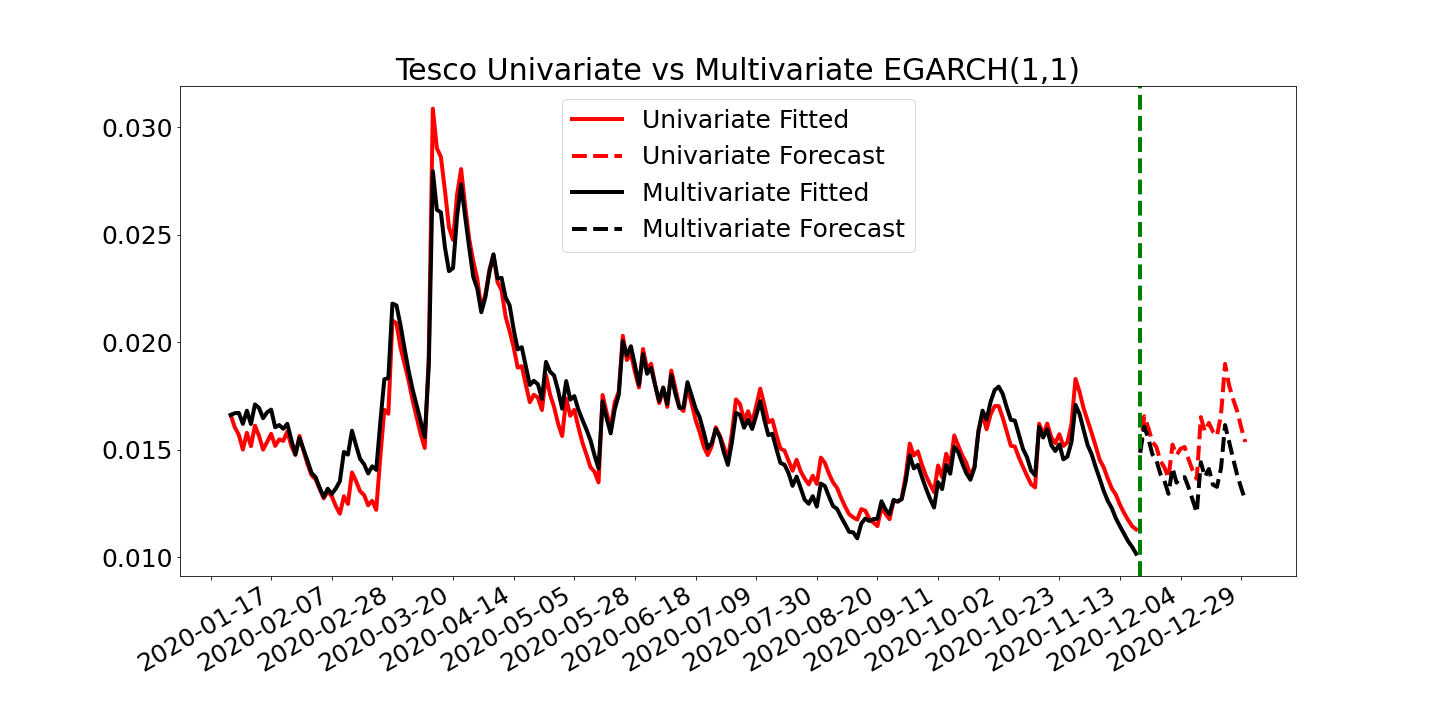
\includegraphics[scale = 0.30]{images/multiGarch/plot 2.png}
\caption{TESCO: Univariate vs Multivariate EGARCH(1,1)}
\label{fig: MV GARCH Example}
\end{figure}

\section{Model Validation}
While I did implement automated model selection methods, these are based on numeric criteria that do not necessarily address all components of a holistic research project. For each hyperparameter I included in my algorithm, I needed to validate the assumptions and limitations of including them in the model, as well as their relative impact on the forecast. 

\subsection{Residual Distributions}
The first hyperparameter I wanted to validate after viewing the grid search output tables was the residual distribution. It was very apparent that in the Tesco and Vodafone models, the students-t distribution was yielding lower values for AIC. I wanted to ensure not only was this accurate, but also there were no better available alternative distributions I could have used. $\mathbf{Figure~4.9}$ was a method used for my validation process, where I, similarly to the distribution of returns, I fit using maximum likelihood estimation, the standardized residuals to multiple distributions. For example, here it was clear why the students-t distribution was performing better than the normal distribution as there was more mass in the tails and a taller peak. I repeated this process with all four stocks optimal models to ensure validity in my residual hyperparameter decision.
\begin{figure}[H]
\centering
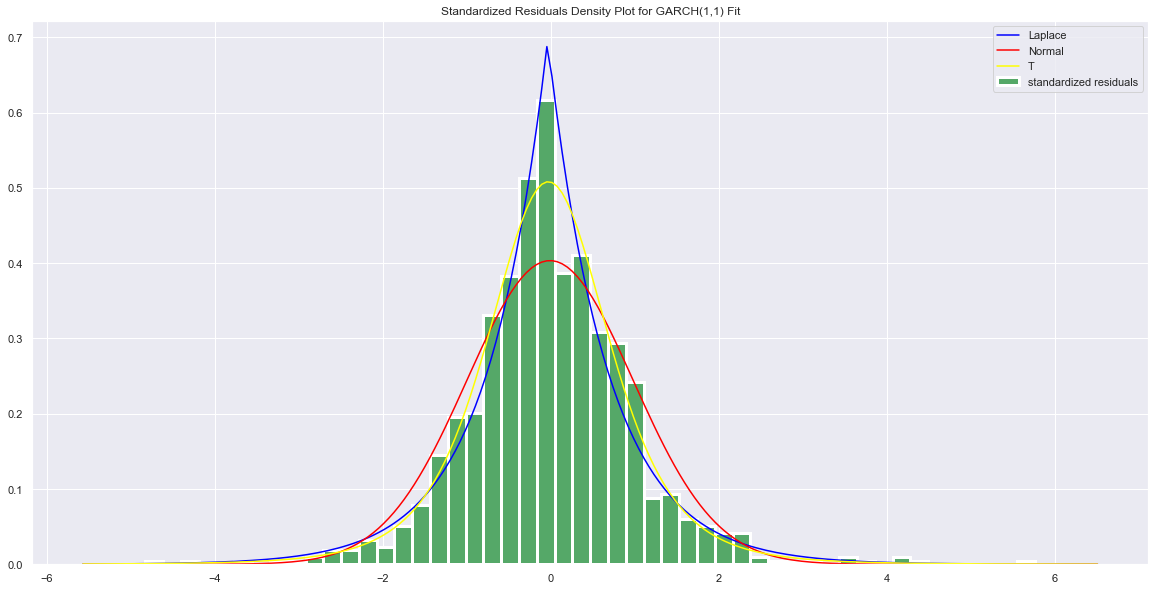
\includegraphics[scale = 0.35]{images/GarchResiduals.png}
\caption{GARCH(1,1) Residuals}
\label{fig: Garch Residuals}
\end{figure}

\subsection{Volatility Model}

I then evaluated why the different volatility models $\mathbf{(EGARCH~vs~GARCH)}$ faired differently. Different from the residual distribution, where a visual test was sufficient to gain understanding and confidence, the answer to this is was found through a better theoretical understanding of the $\mathbf{EGARCH}$ model. According to the creator of the $\mathbf{ARCH}$, Tim Bollserslev \cite{BOLLERSLEV1986307}, he now speaks on the EGARCH: "There is a stylized fact that the EGARCH model captures that is not contemplated by the GARCH model, which is the empirically observed fact that negative shocks at time t-1 have a stronger impact in the variance at time t than positive shocks" \cite{engle} Fundamentally, this concept builds on the older theory of a leverage effect found in a $\mathbf{GJR-GARCH}$. Engle further explained: "negative shock is $\gamma-\alpha$, while the effective coefficient associated with a positive shock is $\gamma+\alpha$. In financial time series, we generally find that $\gamma$ is negative and statistically significant" \cite{engle}. Fundamentally, the $\mathbf{EGARCH}$ model is able to capture the properties of market returns slightly better than the $\mathbf{GARCH}$, and Engle believes this is because the negative shocks have a larger and more significant affect on the next time periods variance than a positive shock. Intuitively this makes sense, as investor behavior tends to be more likely to sell a stock given bad news than buy an equal amount of stock given good news. Given this information I was comfortable with the results of the automated model selection.

\subsection{Lags (p,q)}

Finally, the evaluation of the lag parameters p and q were validated. I approached this problem in two ways, first was through the Partial Autocorrelation Function plots introduced in section one, evaluating the number of lags with significant autocorrelation $mathbf{Figure 4.4}$. This didn't necessarily give an indication of the number of lags the standard deviations had autocorrelation with, but it did give an indicator to the the autocorrelation between the actual time series observations. The second approach was to evaluate the significance of model parameters. In some cases the minimum AIC model would recommend a more complex model, say $\mathbf{EGARCH(3,2)}$, but the parameters for the coefficients of $\alpha_2,~\alpha_3,~\beta_2$ were not significant at the 0.05 level. There is also literature on the topic of models extending the general p=1,q=1 framework, such as Peter Hansen and Asger Lunde's \cite{Hansen11} which explained not only was the forecast accuracy showing no significant difference, but the model complexity actually hurt the analysis not helped. For this reason, whenever I saw a minimal difference in AIC, I always chose the simpler model.  

\subsection{Forecasting}
Since I am focusing on the 1-day ahead "Nowcast" I evaluated two forecasting methods: rolling window and fixed window. The rolling window has a fixed amount of days used in the model, ex: 100 day rolling the model starts on January 1st, uses 100 days of data and forecasts April 11th, the next forecast data begins on January 2nd uses data until April 11th and forecasts April 12th. Conversely, the expanding window forecast continues to aggregate data and the sample used to make the forecast gets larger with each step. An example of the difference in forecasts is shown in $\mathbf{Figure~4.10}$. For this portion of validation there was no objective "better" option, as both have strengths and weaknesses, so I decided to move forward with the forecast method yielding the least generalisation error.  
\begin{figure}[H]
\centering
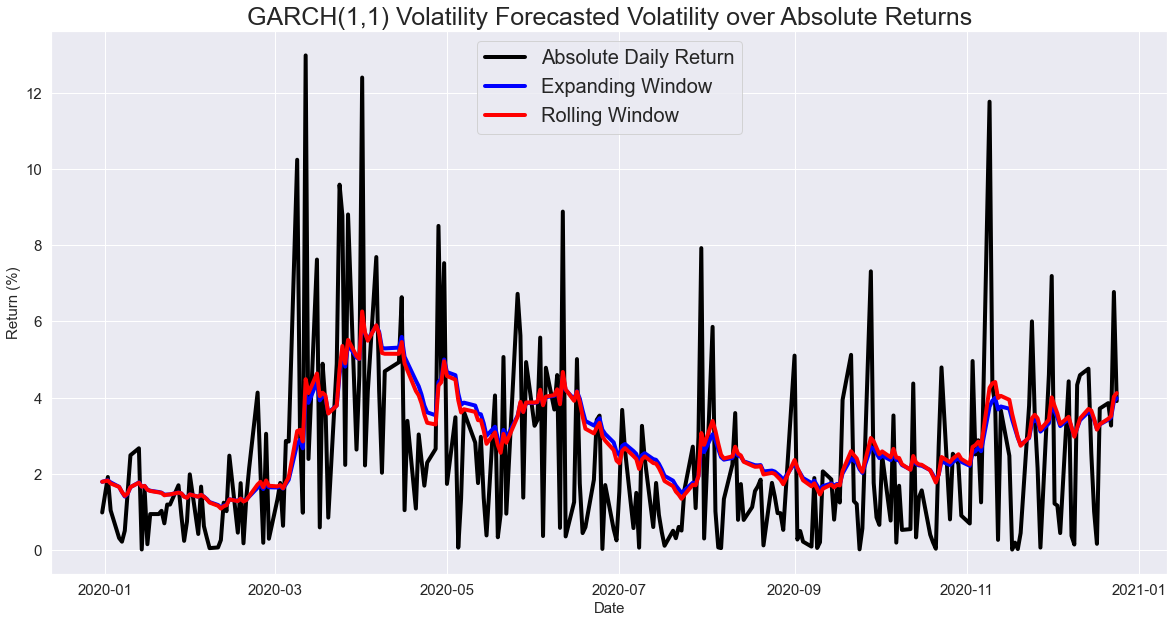
\includegraphics[scale = 0.35]{images/ForecastRollingExpanding1.png}
\caption{Rolling vs Expanding Forecast}
\label{fig: Fitting Plot}
\end{figure}

\section{Model Comparison}
Finally, I needed to determine a consistent method for comparing the accuracy of the forecasts. As noted prior, since it is not possible to extract the exact instantaneous standard deviation from the stock returns, a generally accepted proxy instead is the squared or absolute value of the selected returns, therefore I decided to compare the forecast conditional volatility to squared returns. The comparison was done using two metrics: Mean Absolute Error and Mean Squared Error.
$$
MAE~(Mean~Absolute~Error) = \sum|(\mathbf{X} - \mathbf{\hat{X}})
|$$ $$
MSE~(Mean~Squared~Error) = \sum(\mathbf{X} - \mathbf{\hat{X}})^2$$

The MAE and MSE simply give a generalisation error that can be compared across models to asses accuracy. These metrics will be used on the 1-day ahead rolling forecasts for the 25 day test dataset. 



